\documentclass[10pt,a4paper]{article}
\usepackage[margin=2.2cm]{geometry}
\usepackage{fontspec}
\usepackage{xeCJK}
\setCJKmainfont{SimSun}[BoldFont=SimHei]
\setCJKsansfont{SimHei}
\usepackage{amsmath}
\usepackage{graphicx}
\usepackage{booktabs}
\usepackage{array}
\usepackage{longtable}
\usepackage{caption}
\usepackage{enumitem}
\usepackage{float}
\usepackage[hidelinks]{hyperref}
\setlist{nosep,leftmargin=1.5em}
\setlength{\tabcolsep}{4pt}
\linespread{1.22}
\captionsetup{font=small}
\renewcommand{\figurename}{图}
\renewcommand{\tablename}{表}
\newcolumntype{L}[1]{>{\raggedright\arraybackslash}p{#1}}
\newcommand{\dn}{\Delta n_0}

\title{\textbf{从声光移频器到长孔径分段馈电声光相位调制器：\\思路回顾与主要错误清单}}
\author{陈鑫磊\quad 上海电力大学}
\date{2026 年 10 月 23 日}

\begin{document}
\maketitle

\noindent\fbox{\parbox{\dimexpr\linewidth-2\fboxsep-2\fboxrule}{\small
\textbf{本稿仅限课题组内部：仿真与方案工作稿，实测待做，无伪造数据，Fiber-Q 未下单，无流片；不得作为公开或可引用结果。}
文中器件数字均为 COMSOL 仿真预测或由仿真数据换算，不是实验结果。本稿根据各阶段的 \texttt{summary\_step*.md}、审计记录和工作记录整理，
引用的数字以对应记录文件为准。}}

\section{一句话总结}
最初的方案是“双环光子分子 + 悬空叉指换能器”的谐振式声光移频器（预印本声称 98.3\% 移频效率、6.7 µW 驱动）。
10 月 16 日用本结构做光弹实算，发现单位电压的驱动强度只有 1.65 MHz/V，比方案里借用的 21.3 GHz/V 低约 $1.3\times10^4$ 倍，
移频器方案就此放弃。之后转向“把光波导放进叉指孔径内部”的行波声光相位调制器，经过一系列数值与建模排查
（单元阶次、二维/三维一致性、张量取向、接地、单位、认模），再到器件层面的功率、超胞、取向和匹配问题，
最终形成现在的版本：\textbf{Shao 型晶体取向、400 nm 脊、100 µm 分段、串并联配 50 Ω、带支撑梁和引线}，
$L = 1$ mm 信号源功率仿真约 3.3 mW（乘校准系数后 5.5–17 mW）。图~\ref{fig:hist} 给出这一过程中功率预测的变化。

\begin{figure}[H]
\centering
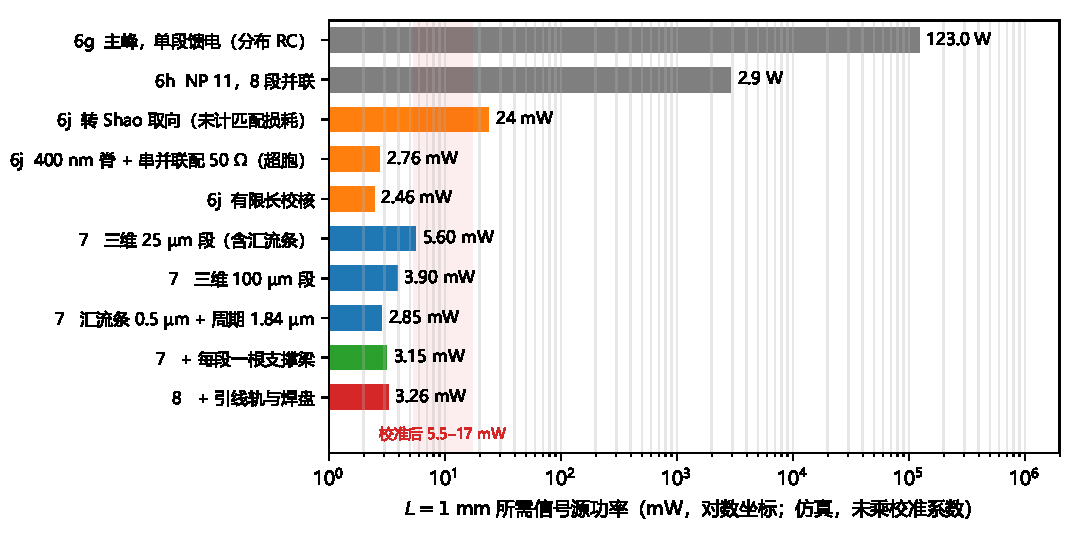
\includegraphics[width=0.95\linewidth]{fig_history.pdf}
\caption{相位调制器阶段 $L = 1$ mm 所需信号源功率的演变（仿真，未乘校准系数）。灰色：旧取向、单段或少段馈电；
橙色：二维截面优化后；蓝色：三维分段模型；绿/红：加入支撑梁和引线。移频器阶段的指标不同（单位电压的移频驱动强度），未画入。}
\label{fig:hist}
\end{figure}

\section{思路演变（按时间）}

\subsection{阶段 0：谐振式声光移频器（约 10 月 7–15 日）}
\begin{itemize}
\item \textbf{方案}：单总线耦合的双环（光子分子），环 1 约 15\% 周长上方是悬空叉指声学谐振腔（3.33 GHz）。
声波调制使光在两个超模之间跃迁，实现单边带移频；理论框架用 Hu 2021 的耦合模方程。
\item \textbf{关键假设}：驱动强度 21.3 GHz/V，由 Shao 2019 的 $V_\pi L = 0.046$ V$\cdot$cm 外推而来，不是本结构算出的。
\item \textbf{当时的结论}：98.3\% 移频、6.7 µW 驱动、蒙特卡罗良率 96.4\%，写成预印本草稿（10 月 14 日）。
\item \textbf{复现与审计}（10 月 7 日、15 日）：发现手册变量标反、文献点画错坐标轴、蒙特卡罗靠收紧假设才过线、
相对电光方案的功率优势被夸大（未匹配电光作对比）等问题，逐项改正（见表~\ref{tab:err} 第 2、3、25 条）。
\end{itemize}

\subsection{阶段 1：光弹实算，放弃移频器（10 月 16 日）}
用本结构的 1 V 压电 + 光弹仿真直接计算驱动强度：1.65 MHz/V，比假设低约 $1.3\times10^4$ 倍；要达到原指标需约 300 V。
在可行窗口内最好也只有约 1.58 GHz/V、对应约 1.2 mW。结论是谐振移频器在本结构下不成立，方案放弃，数据保留。
这一步的教训贯穿后面全部工作：\textbf{借来的实验标定必须用本结构的有限元结果复核}。

\subsection{阶段 2：孔径内声光调制的预研、审计与矢量光学基线（10 月 16–21 日）}
中间短暂讨论过其他方向（量子、量子点路由、平台比较），与本课题无关，不展开。随后回到悬空叉指，
把光波导放在叉指孔径内部，做孔径宽度扫描与声光重叠，整理成预印本包（10 月 21 日）。
对这个包做的审计推翻了几项结论：6 µm 孔径“最优”的排序被网格加密推翻；耦合声模频率未收敛；“移频”措辞过度。
同期做的矢量光学基线发现铝损耗符号写反、贴铝布局下没有可用光模、各向异性设置有误；模式跟踪工具本身也有多处错误。
这一阶段的结论基本都被撤回，留下的是“需要一套可核对的二维/三维流程”这一需求。

\subsection{阶段 3：数值与建模排查，Step 1–5（10 月 21 日）}
目标是让二维截面与三维模型给出一致的声学频率和压电场，作为后续一切计算的基础。
\begin{itemize}
\item Step 1：三维用一阶单元时频率偏差 $-1162$ MHz，改二阶后仍差 $+230$ MHz；
\item Step 2：二维 PlaneStrain 等价于强制 $w=0$，丢掉了面外位移（约 35.6 MHz）；
\item Step 3：二维材料张量的基矢取向错误，$c^E$ 等分量相差 16–200\%，改用 \texttt{sys2} 并在每次运行打印张量检查；
\item Step 4：接地边按“相交”选择会多选 5 条边（约 48 MHz）；改正后二维与三维频率一致到 0.01\% 以内，周期定为 2.8526 µm；
\item Step 5：驱动响应与相位计算（其中有单位错误，见表~\ref{tab:err} 第 19 条，到 6a 才改正）。
\end{itemize}

\subsection{阶段 4：孔径内相位调制器原型，Step 6a–6e（10 月 21–22 日）}
引入光学模式，计算声致折射率变化 $\dn$ 与 $V_\pi L$。期间修正了归一化、认模（必须按铝中能量占比 fracAl 认模，
不能按频率最近）、TM 参考折射率等问题；发现沟槽脊方案光学泄漏不可用，改为标准脊（平板 400 nm，缺陷胞 3 个）；
确定周期 2.71043685 µm。6e 得到 $V_\pi L \approx 0.87$ V$\cdot$cm，第一次有了完整的器件数字。

\subsection{阶段 5：功率与超胞问题，Step 6f–6h（10 月 22 日）}
\begin{itemize}
\item 6f 算功率时只看了 $V_\pi$，一个低频峰看起来“好 5.8 倍”；
\item 6g 加入电极分布电阻后发现电阻占功率的 85–99\%，集总模型不成立，$L = 1$ mm 主峰需要 123 W；
\item 6h 发现低频峰是周期超胞的能带折叠假象，“亚瓦”标题撤回；超胞结果对缺陷胞数 NP 不收敛；分段并联后最低约 2.9 W（$L=1$ mm）。
\end{itemize}
到这里功率仍在瓦级，比 Shao 等已发表器件差一个数量级以上。

\subsection{阶段 6：文献对照与校准，Step 6h\_lit、6i（10 月 22 日）}
与 Shao 2019 对比，本结构 $V_\pi L$ 差 16–19 倍。为了区分“模型误差”和“结构差距”，用同一流程重算 Shao 的结构做校准。
第一次校准因坐标旋转方法（\texttt{inPlane}）错误而作废，改为 \texttt{general} 重算后得到：本流程 $\dn$ 偏高 1.3–2.3 倍，
即功率需乘 1.7–5.3 倍。说明主要差距来自结构本身，而不是模型。

\subsection{阶段 7：取向、脊高与匹配，Step 6j（10 月 22 日）}
找到结构差距的主因：旧取向下可用的光弹/电光系数很小。改用 Shao 型取向后效率提高约 220 倍，400 nm 脊再提高约 7 倍。
同时发现“无损匹配”假设（0.7–1.4 Ω 对 50 Ω）不现实，改为多段串并联直接配 50 Ω；超胞 1.8 倍的分散用有限长模型核对。
$L = 1$ mm 功率降到约 2.5–2.8 mW（二维）。另做了新颖性检查（Freedman 2025 最接近，但结构与指标不同）。

\subsection{阶段 8：三维分段与可加工性，Step 7–9（10 月 22–23 日）}
\begin{itemize}
\item Step 7：三维分段模型显示汇流条与指端会引起模式分裂，25 µm 段损失 2–2.6 倍；改为 100 µm 段、0.5 µm 汇流条后只差 1.10 倍；
周期按线性斜率 $-1.33$ MHz/nm 调到 1.84 µm。每段加一根支撑梁，幽灵几何对照证实 1.11 倍是物理效应，梁端 PML 与固定端差 $<1\%$。
\item Step 8：两侧引线轨增加 3–4\%，空气桥光吸收可忽略，$L = 1$ mm 约 3.26 mW。
\item Step 9：悬空段与普通波导之间的光学过渡，二维模式匹配约 0.025 dB/个，可忽略。
\end{itemize}

\subsection{当前版本与未覆盖项}
当前版本：Shao 型取向，400 nm 脊，周期 1.84 µm，100 µm 分段，0.5 µm 汇流条，每段一根支撑梁，两侧引线，串并联配 50 Ω。
$L=1$ mm 信号源功率 3.26 mW（仿真）/ 5.5–17 mW（校准后）。流片前仍需：版图（GDS）、按工艺参数重算（A3）、机械可行性（A7），
以及沿波导方向的声学端部、三维释放边缘等尚未覆盖的问题（详见 \texttt{report\_summary.pdf}）。

\section{主要错误与处理}
表~\ref{tab:err} 按类型列出主要错误。“发现方式”一栏中“用户”指由陈鑫磊审阅时指出。

{\small
\begin{longtable}{>{\raggedright\arraybackslash}p{0.45cm}L{3.7cm}L{2.7cm}L{3.5cm}L{4.4cm}}
\caption{主要错误、发现方式、影响与处理（方括号内为阶段）}\label{tab:err}\\
\toprule
\# & 问题 & 发现方式 & 影响 & 处理 \\
\midrule
\endfirsthead
\toprule
\# & 问题 & 发现方式 & 影响 & 处理 \\
\midrule
\endhead
\bottomrule
\endfoot
\multicolumn{5}{l}{\textbf{A. 方案与物理层面（导致方向改变）}}\\
1 & [移频器] 驱动强度 21.3 GHz/V 借用 Shao 2019 外推，未在本结构上验证 & 1 V 光弹实算 & 实际 1.65 MHz/V，差约 $1.3\times10^4$ 倍；全部移频指标不成立 & 放弃移频器方案，数据保留；此后所有驱动量都用本结构有限元计算 \\
2 & [移频器] 相对电光方案的功率优势被夸大 & 复现审计 & 宣称的优势从 $1.3\times10^4$ 倍降到 440 倍，再降到 1.4–3.7 倍 & 对比对象改为已匹配的电光器件，按实际数字表述 \\
3 & [移频器] 蒙特卡罗良率 96.4\% 靠收紧假设得到，无对应样本 & 复现审计 & 良率被高估 & 改用有样本支撑的 94.3\%；补充耦合间隙 $\sigma = 5$ nm 引起约 114 MHz 劈裂分散 \\
4 & [6h] 低频峰“亚瓦”实为超胞能带折叠假象 & 有限长与 NP 扫描 & “亚瓦”标题错误 & 撤回；此后周期超胞结论都用有限长模型核对 \\
5 & [6h→6j] 旧晶体取向下可用系数很小 & 与 Shao 对比、校准后排除模型误差 & $V_\pi L$ 比 Shao 差 16–19 倍 & 改 Shao 型取向（约 220 倍）+ 400 nm 脊（约 7 倍） \\
6 & [6f] 功率只按 $V_\pi$ 算，未计电极电阻 & 6g 分布 RC 模型 & 电阻占 85–99\%，功率低估一个数量级以上 & 改用分布 RC/传输线模型，功率一律算到 50 Ω 信号源 \\
7 & [6j] “无损匹配”假设（0.7–1.4 Ω 配 50 Ω） & 估算匹配网络损耗 & 功率过于乐观 & 改为多段串并联直接配 50 Ω \\
8 & [7] 二维截面忽略汇流条和指端 & 三维分段模型 & 25 µm 段损失 2–2.6 倍 & 段长 100 µm、汇流条 0.5 µm，损失降到 1.10 倍（1 µm 汇流条会与旁模合并，不采用） \\
\midrule
\multicolumn{5}{l}{\textbf{B. 建模与数值}}\\
9 & [Step 1] 三维一阶单元、网格粗 & 二维/三维对照 & 频率偏 $-1162$ MHz；早期“必须悬空”等判断很可能部分基于此 & 改二阶单元并加密；早期三维结论重新核对 \\
10 & [早期] 漏掉压电电荷守恒（出现两次） & 复核模型设置 & 压电场错误 & 补上电荷守恒，加入检查项 \\
11 & [Step 2] 二维与三维周期不一致（2.58 vs 2.8326 µm）；PlaneStrain 等价 $w=0$ & 逐项对照 & 二维/三维不可比，约 35.6 MHz 偏差 & 统一周期；改用面外扩展（ModeExtension） \\
12 & [Step 3] 二维材料张量基矢取向错误 & 打印张量对比 & $c^E$ 等分量差 16–200\% & 改用 \texttt{sys2}，每次运行打印张量检查 \\
13 & [Step 4] 接地边按“相交”选择，多选 5 条边 & 打印选中边 & 约 48 MHz 偏差 & 改精确选择并打印检查；二维/三维一致到 0.01\% \\
14 & [6i] 坐标旋转用 \texttt{inPlane}，旋转被截断 & 张量检查与结果异常 & 第一次 Shao 校准作废 & 改 \texttt{general} 重算（提交 3e9b2b3 → fba4d2d） \\
15 & [6h/6j] 周期超胞结果对 NP 不收敛 & NP 扫描 & 超胞结果分散 1.8 倍以上 & 用有限长模型作为基准 \\
16 & [6j] 周期按 $f\propto1/p$ 估算 & Step 7 实算 & 估到 1.86–1.89 µm，实际应为 1.84 µm & 改用实测线性斜率 $-1.33$ MHz/nm（\texttt{summary\_step6j.md} 尚未标注） \\
17 & [6b2] TM0 参考值按各向同性给出（1.7432） & 各向异性复算 & 参考值偏差，对结果影响 $<1\%$ & 更正为 1.718502 \\
18 & [6c] 沟槽脊横向泄漏；贴铝平板无可用光模 & 光学模式计算 & 方案光学上不可行 & 改标准脊（平板 400 nm，缺陷胞 3 个） \\
\midrule
\multicolumn{5}{l}{\textbf{C. 后处理、单位与判定}}\\
19 & [Step 5] 相位 $\phi/L$ 换算因子写成 $\times1000$（应 $\times10^{-3}$） & 6a 自检 & 数值偏大 $10^6$ 倍 & 6a 起改正（\texttt{postprocess\_6a.py}“修正 1”）；\texttt{summary\_step5.md} 尚未标注 \\
20 & [6a/6b1] 归一化缩放错误 & 自检对照 & 旧的谐波结果无效 & 统一归一化后重算 \\
21 & [6c] 伙伴模认错（按频率最近认模） & 用户 & 合格判断从“合格”变为“不合格” & 统一按铝中能量占比 fracAl 认模 \\
22 & [6e] 扫描参数应填 $\beta$ 却填了别的量；首轮扫描窗口错过峰值 & 结果异常、加宽窗口 & 出现伪模，峰值漏掉 & 改为 $\beta$，扩大窗口重扫 \\
23 & [基线] 铝损耗虚部符号写反（$+15.6i$） & 审计 & 铝变成增益介质 & 改为 $-15.6i$ \\
24 & [审计工具] 重叠指标无界、参数错位、导出路径错、加密出现“假平台” & 审计复核 & 相关结论不可靠 & 撤回对应结论；修正工具后重算 \\
25 & [移频器] 手册变量 $c_1$/$m_1$ 标反；文献点画错坐标轴 & 复现 & 效率显示 0.75\%（应为 98.31\%） & 更正标注和图 \\
\midrule
\multicolumn{5}{l}{\textbf{D. 表述与判断（审阅中纠正）}}\\
26 & “串联段越多越敏感” & 用户 & 结论方向错误 & 按实际电路关系改写 \\
27 & “2 MHz 约对应 2 nm” & 用户 & 工艺容差估计偏紧 & 更正为约 4.7 nm \\
28 & “校准系数与三维损失重复计算” & 复核 & 低估功率 & 两者独立，可以直接相乘 \\
29 & 梁端用固定边界 & 用户（固定边界会全反射） & 可能高估梁的影响 & 改 PML，对照固定端差 $<1\%$ \\
30 & 梁的 1.11 倍疑为网格效应 & 幽灵几何对照 & — & 对照逐位一致，确认为物理效应 \\
31 & “周期扫描最重要”“目前没问题可以流片” & 复核 & 优先级与成熟度表述过头 & 更正，并列出流片前未覆盖的项目 \\
\midrule
\multicolumn{5}{l}{\textbf{E. 工具与流程事故}}\\
32 & 中文报告被 PowerShell 以错误编码写入 & 打开乱码 & 文件不可恢复 & 重写；之后只用文件工具写文本 \\
33 & Step 9 日志与 COMSOL 日志仅大小写不同，Windows 下互相覆盖 & 日志缺失 & COMSOL 日志被删 & 改名 \texttt{step9\_match.log}，重跑得到同样数字 \\
34 & Step 9 批处理模式下 \texttt{args} 为空导致空指针；加密参数被覆盖 & 运行报错 & 加密算例未执行 & 判空，单独生成加密版本类 \\
35 & 25 µm 段大模型内存不足；Step 8 选择标签写错；分散脚本遇空值 & 运行报错 & 算例中断 & 重跑、修标签、对空值截断处理 \\
\end{longtable}
}

\section{经验与固定下来的做法}
\begin{enumerate}
\item \textbf{借用的数字必须在本结构上复算}：移频器的失败就在于驱动强度来自外推（差 $1.3\times10^4$ 倍）。
\item \textbf{每次运行打印自检}：材料张量、接地边、旋转方法、单位换算都在日志里输出，便于复核（Step 3、4、5、6i 的错误都靠这个发现）。
\item \textbf{认模按物理量}：用铝中能量占比、场分布认模，不按频率最近。
\item \textbf{周期模型要用有限长核对}：超胞会产生折叠峰，且对缺陷胞数不收敛。
\item \textbf{功率算到 50 Ω 信号源}：包含电极电阻、匹配方式和三维损失，否则会差一到几个数量级。
\item \textbf{用已发表结构校准}：同一流程算 Shao 的结构，把“模型误差”与“结构差距”分开。
\item \textbf{区分数值与物理}：网格加密、幽灵几何、边界条件对照（PML 与固定端）。
\item \textbf{表述保守}：数字一律标明“仿真预测”；作废的结论在原记录中标注，不静默删除。
\end{enumerate}

\section{原记录中尚未标注的更正}
\begin{itemize}
\item \texttt{step5\_drive/summary\_step5.md}：$\phi/L$ 偏大 $10^6$ 倍的问题（第 19 条）未在该文件中标注，正确值以 6a 为准。
\item \texttt{step6\_optics/summary\_step6j.md}：按 $f\propto1/p$ 估的周期 1.86–1.89 µm（第 16 条）未更正，正确值见 Step 7（1.84 µm）。
\end{itemize}

\end{document}
